\subsection*{Temporal Ontology in the Vortex Æther Model}

Before deriving explicit time dilation relations, we summarize the key modes of time present in VAM, which reflect different physical aspects of vortex structures and æther flow. These temporal quantities appear in various field equations and define how duration and simultaneity are treated in the model.

\begin{center}
\begin{tcolorbox}[
  colback=gray!10,
  colframe=black,
  width=0.9\textwidth,
  sharp corners=southwest,
  boxrule=0.5pt,
  before skip=10pt,
  after skip=10pt,
  title=\textbf{Table: Ætheric Time Modes in the Vortex Æther Model},
  fonttitle=\bfseries,
]
\renewcommand{\arraystretch}{1.25}
\begin{tabularx}{@{}lll@{}}
  \(\mathcal{N}\)     & \textbf{Aithēr-Time}         & Absolute causal background \\
  \(\nu_0\)           & \textbf{Now-Point}           & Localized universal present \\
  \(\tau\)            & \textbf{Chronos-Time}        & Measured time in the æther \\
  \(S(t)\)            & \textbf{Swirl Clock}         & Internal vortex phase memory \\
  \(T_v\)             & \textbf{Vortex Proper Time}  & Circulation-based duration \\
  \(\mathbb{K}\)      & \textbf{Kairos Moment}       & Topological transition point \\
\end{tabularx}
\end{tcolorbox}
\end{center}

\phantomsection
\label{tab:ÆtherTimeModes}



These distinct time concepts clarify how local and global phenomena are distinguished within VAM, providing a basis for the derivation of time dilation below.



\section*{Scale-dependent Æther Densities in VAM}


The Vortex Æther Model distinguishes between two conceptually distinct densities:

\begin{itemize}
    \item \textbf{Æther Fluid Density} \(\rho_{\text{\ae}}^{\text{(fluid)}}\) — a constant background value (\(\sim 7 \times 10^{-7}\, \mathrm{kg/m^3}\)) that governs wave propagation and inertial resistance at macroscopic scales.
    \item \textbf{Æther Mass-Energy Density} \(\rho_{\text{\ae}}^{\text{(mass)}}(r)\) — a radially decaying field around vortex cores responsible for storing rotational energy and generating topological stability.
\end{itemize}

The energy density is high near vortex cores (\(\sim 10^{18}\, \mathrm{J/m^3}\)) and decays exponentially toward the fluid density background on
macroscopic scales.


\subsection*{1. Fluid Density: Constant Background}

The æther fluid density is taken to be approximately:
\begin{equation}
    \rho_{\text{\ae}}^{\text{(fluid)}} \approx \SI{7e-7}{kg/m^3},
\end{equation}
based on matching vortex energetics with known quantum properties and allowing for inertia-free propagation of signals in the far field.

\subsection*{2. Energy Density: Core-Localized}

In contrast, the energy density near a vortex core satisfies:
\begin{equation}
    \rho_{\text{\ae}}^{\text{(energy)}}(r \to 0) \sim \SI{3.89e18}{J/m^3},
\end{equation}
which is necessary to stabilize the core topology. This follows from the vortex energy expression:
\begin{equation}
    E_{\text{vortex}} = \frac{1}{2} \rho_{\text{\ae}}^{\text{(energy)}} \Omega^2 r_c^5
    \quad\Rightarrow\quad
    \rho_{\text{\ae}}^{\text{(energy)}} \sim \frac{2E}{\Omega^2 r_c^5},
\end{equation}
where \( \Omega = \frac{C_e}{r_c} \), with \( C_e \approx \SI{1.093845e6}{m/s} \) and \( r_c \approx \SI{1.40897e-15}{m} \).

\subsection*{3. Transition Profile}

The energy density transitions exponentially to the macroscopic background:
\begin{equation}
    \rho_{\text{\ae}}^{\text{(energy)}}(r) =
    \rho_{\text{\ae}}^{\text{(fluid)}} +
    \left(\rho_{\text{core}} - \rho_{\text{\ae}}^{\text{(fluid)}}\right)
    e^{-r/r_*},
\end{equation}
where \( r_* \sim \SI{1e-12}{m} \) represents the characteristic decay scale of vortex influence.

\begin{figure}[htbp]
    \centering
    \includegraphics[width=0.85\textwidth]{images/00_scaleDependentÆtherDensity}
    \caption{Energy density in the æther decreases exponentially from the vortex core and asymptotically reaches the macroscopic fluid density.}
    \label{fig:vortexfields2}
\end{figure}

\begin{table}[h!]
    \centering
    \begin{tabular}{|c|c|c|l|}
        \hline
        Regime & Distance $r$ & $\rho_{\text{\ae}}^{\text{(energy)}}(r)$ & Interpretation \\
        \hline
        Core & $r < 10^{-14}$ m & $\sim 10^{18}$ J/m$^3$ & Topological vortex energy \\
        Transition & $10^{-14}$–$10^{-11}$ m & Exponentially decreasing & Energy storage / swirl gradient \\
        Macroscopic & $r > 10^{-11}$ m & $\sim 10^{-7}$ kg/m$^3$ & Baseline fluid density \\
        \hline
    \end{tabular}
    \caption{Behavior of the æther energy density across regimes. The fluid density remains constant.}
\end{table}

\begin{tcolorbox}[colback=blue!3, colframe=black!70, sharp corners=southwest, title=Æther Density Types in VAM]
    \begin{itemize}
        \item \textbf{Fluid Density} \(\rho_{\text{\ae}}^{\text{(fluid)}} \sim \SI{7e-7}{kg/m^3}\): constant across all scales; governs inertia and wave propagation.
        \item \textbf{Energy Density} \(\rho_{\text{\ae}}^{\text{(energy)}}(r)\): concentrated around vortex cores; provides topological stability; decays exponentially:
        \[
            \rho_{\text{\ae}}^{\text{(energy)}}(r) = \rho_{\text{\ae}}^{\text{(fluid)}} + \left(\rho_{\text{core}} - \rho_{\text{\ae}}^{\text{(fluid)}}\right) e^{-r/r_*}
        \]
    \end{itemize}
\end{tcolorbox}


\section{Layered Time Dilation from Swirl Dynamics}

In the Vortex Æther Model (VAM), time unfolds through multiple physical layers, as summarized earlier in the Ætheric Time Modes (see Table~\ref{tab:ÆtherTimeModes}). Absolute time \(\mathcal{N}\) flows uniformly across the æther, while localized structures such as vortex knots experience time differently — through internal swirl clocks \(S(t)\), vortex proper time \(T_v\), and observer-perceived time \(\tau\).


We consider an invisible, irrotational superfluid æther hosting stable, knotted vortex structures. The absolute time \(\mathcal{N}\) flows uniformly across the entire medium, but clocks embedded within vortex regions experience slowed progression, governed by the local vortex velocity field \(v_\varphi(r)\).

This yields a distinction between the global time \(\tau\), the local swirl clock \(S(t)\), and the vortex proper time \(T_v\), each tracing different aspects of duration. The essence of time dilation in VAM is the reduction in local clock rate as a function of rotational energy density and internal circulation of the æther.


\begin{figure}[htbp]
    \centering
    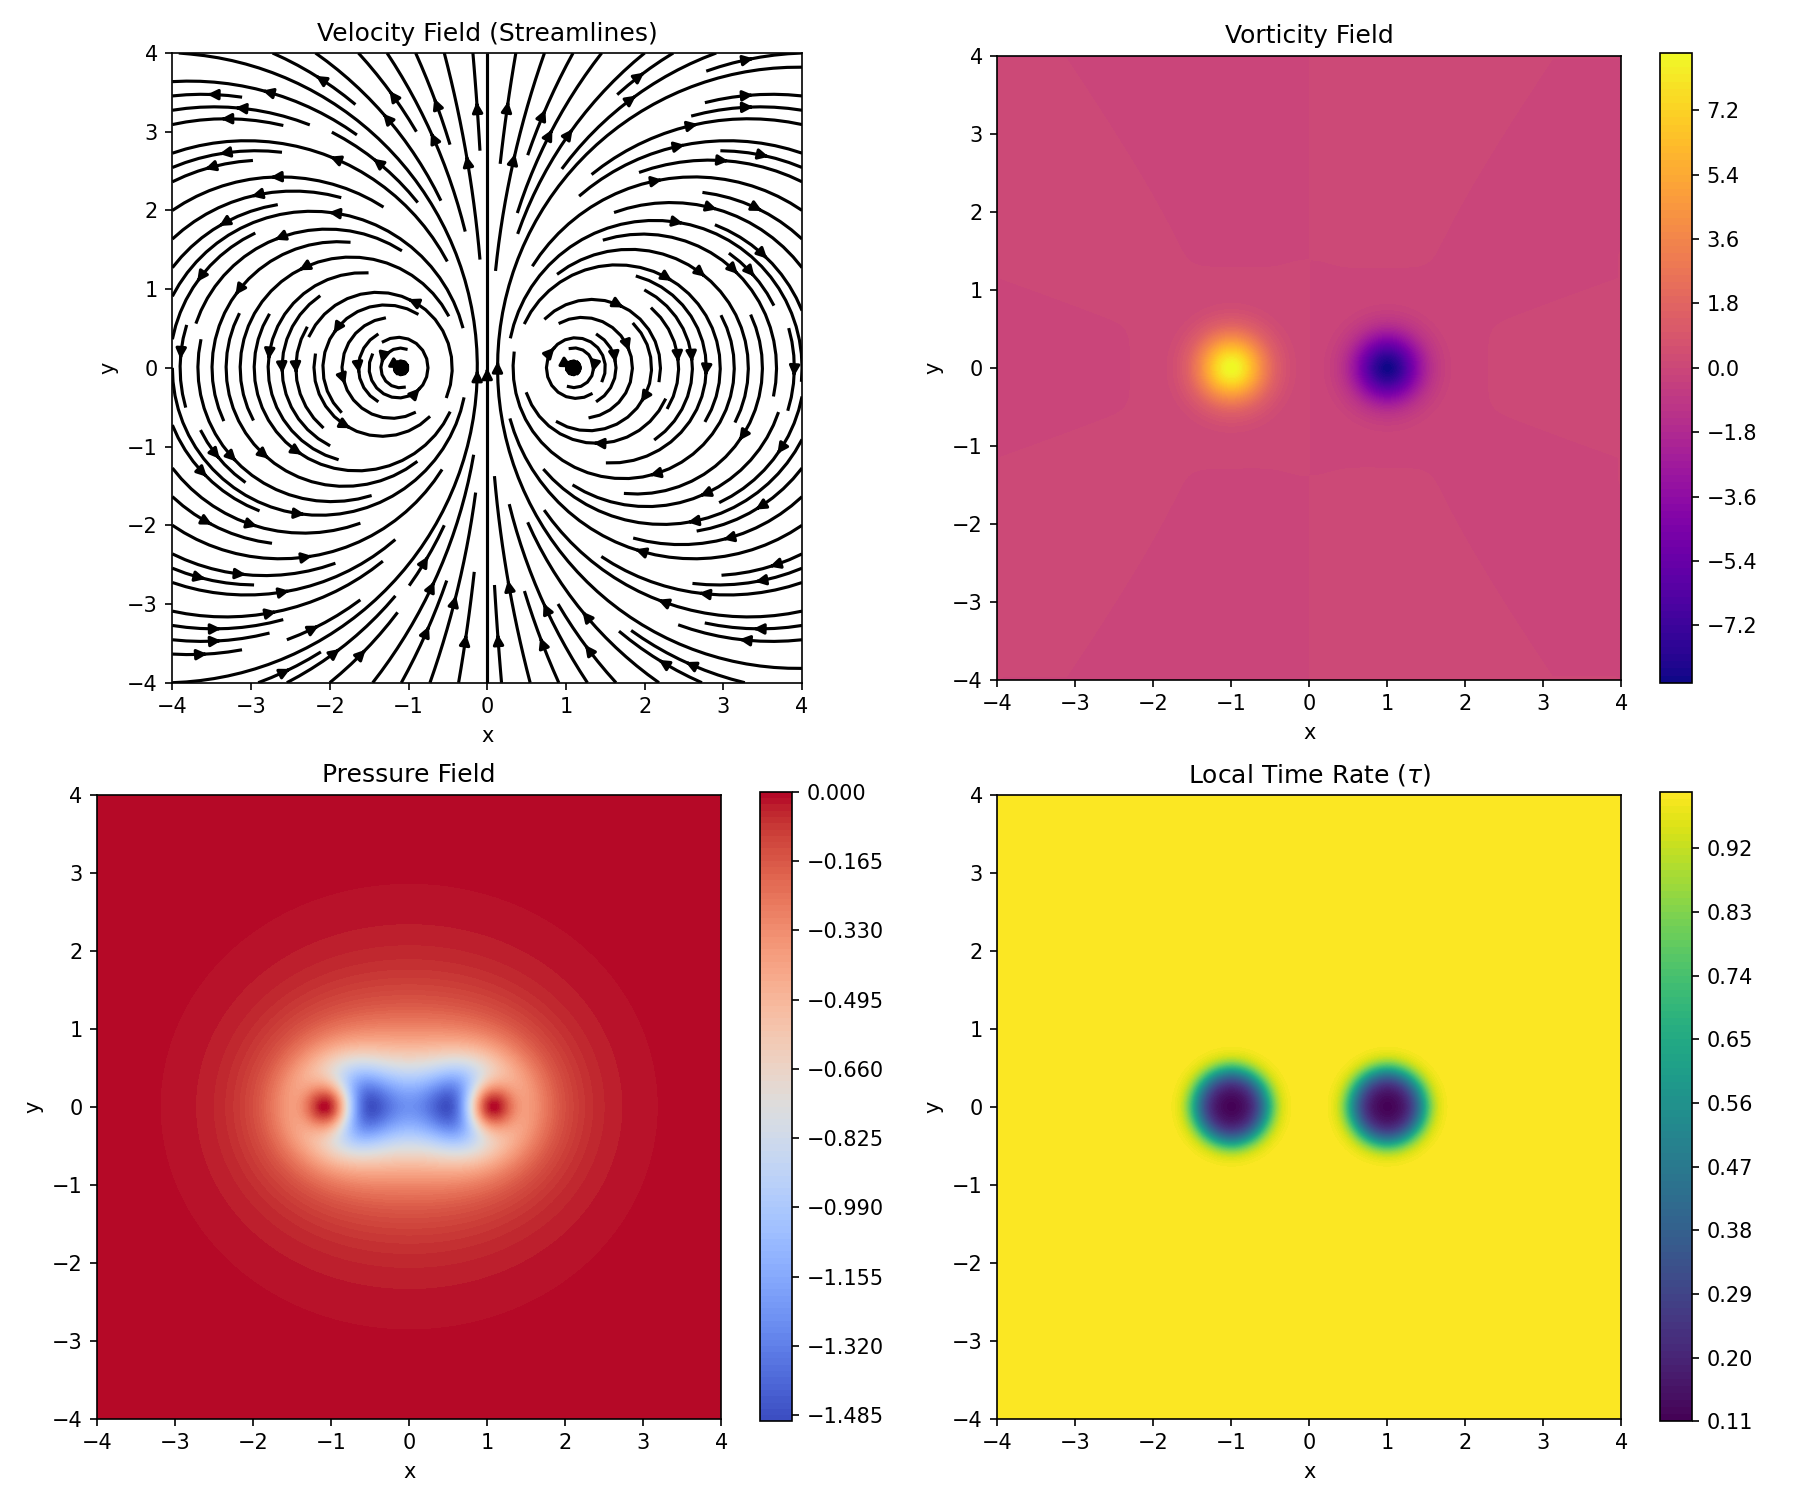
\includegraphics[width=0.85\textwidth]{images/01-streamlinesDiPole}
    \caption{Velocity streamlines, vorticity, pressure and local time velocity $\tau$ for a simulated vortex pair. The pressure minimum and the time delay clearly correspond to the regions of high vorticity. This immediately illustrates the central claim of the Æther model: time dilation follows from vortex energetics and pressure reduction.}
    \label{fig:vortexfields}
\end{figure}

In the Vortex Æther Model (VAM), time dilation does not arise from the curvature of spacetime, but from local vortex dynamics. Each particle of matter in VAM is a vortex-node structure whose internal rotation (\textit{swirl}) influences the local clock frequency.

The fundamental link between local vortex velocity and local time measurement follows from the Bernoulli-like relation for pressure reduction in flow fields. This local time $\tau$ is distinct from both the global causal time $\mathcal{N}$ and the far-field observer’s external time $\bar{t}$. The dilation arises from the slowdown of $\tau$ relative to both $\bar{t}$ and $\mathcal{N}$ as rotational energy increases. See Equation~\eqref{eq:vortex_time_explicit} and the generalized frequency-based dilation formula $\frac{d\tau}{d\bar{t}} = \omega_{\text{obs}}/\omega_0$.  The local clock frequency is related to the vortex tangential velocity $v_{\phi}(r)$ by the formula:
\begin{equation}\label{eq:vortex_time_dilation}
\frac{d\tau}{dt} = \sqrt{1 - \frac{v_{\phi}^2(r)}{c^2}}
\end{equation}

Where $v_{\phi}(r)$ is the tangential velocity of the æther medium at distance $r$ from the center of the vortex, and $c$ is the speed of light. This is a direct analogy with the special relativistic velocity-dependent time dilation, but without spacetime curvature and caused solely by local rotation of the æther medium.

To visualize the outer behavior of time dilation predicted by the heuristic vortex-induced model, we extend the radial domain up to macroscopic femtometer scales. This reveals the asymptotic behavior of time rate restoration in the far-field, confirming agreement with known gravitational time dilation decay profiles.

\begin{figure}[H]
    \centering
    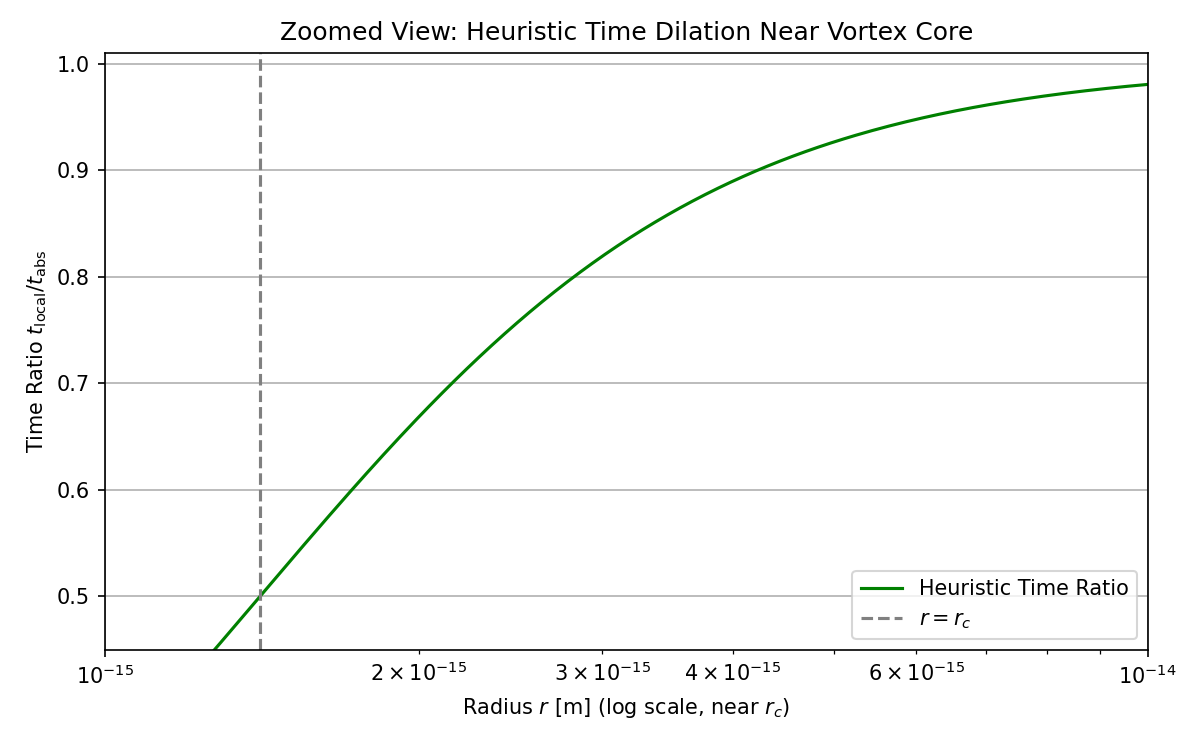
\includegraphics[width=0.7\textwidth]{images/06-HeuristicTimeDilation4}
    \caption{
        Zoomed radial profile of vortex-induced time dilation near the core.
        This heuristic plot illustrates how the normalized local clock rate
        $\frac{d\tau}{dt}$ rapidly increases with distance $r$ away from the core,
        approaching unity asymptotically. This directly visualizes the effect of
        tangential vortex velocity $v_\varphi(r) \sim \kappa / r$ on the local time flow,
        as predicted by equation\eqref{eq:vortex_time_explicit}.
    }
    \label{fig:HeuristicTimeDilation}
\end{figure}


To formalize the distinct temporal flows in the Vortex Æther Model (VAM), we define the following expressions for time accumulation:

\begin{align}
    S(t) &= \int_0^t \Omega(r(t'))\, dt'
    && \text{(Swirl Clock: internal phase accumulation)} \\
    T_v &= \oint \frac{dl}{v_\varphi(r)}
    && \text{(Vortex proper time: loop integral over local swirl speed)} \\
    \frac{d\tau}{dt} &= \sqrt{1 - \frac{v_\varphi^2(r)}{c^2}}
    && \text{(Time dilation from tangential vortex flow)}
\end{align}

Here, \(\Omega(r) = \frac{C_e}{r_c} e^{-r/r_c}\) is the local swirl angular velocity, and \(v_\varphi(r) = C_e e^{-r/r_c}\) the tangential velocity in the æther vortex.

If the swirl is stable and constant at radius \(r\), the swirl clock becomes periodic:
\[
    S(t) = \Omega(r) t \bmod 2\pi
\]
encoding a persistent memory of internal vortex phase.

\begin{tcolorbox}[colback=gray!5, colframe=black!70, sharp corners=southwest, title=Temporal Phase vs. Duration]
    While \(T_v\) measures elapsed duration along the vortex loop (akin to proper time), the swirl clock \(S(t)\) accumulates internal phase, encoding rotational memory modulo full revolutions. This distinction mirrors that between a watch counting seconds and a gyroscope preserving orientation — both describe time, but with fundamentally different informational content. In systems with quantized circulation, such as knotted vortex cores, \(S(t)\) may serve as a persistent state variable marking phase-locked synchronization with external æther flows.
\end{tcolorbox}


\noindent
These temporal flows distinguish between the \emph{absolute æther time} (\(\mathcal{N}\)), the \emph{external observer’s clock} (\(\tau\)), and the \emph{internal vortex timing} (\(S(t)\), \(T_v\)). Their interaction forms the backbone of time dilation and causality in the VAM — not as a deformation of spacetime, but as a direct expression of circulation, angular momentum, and vortex topology.

\medskip
To relate Chronos-Time $\tau$ to externally measured coordinate time $\bar{t}$, we introduce a frequency ratio expression based on the local swirl profile:

\begin{equation}
    \frac{d\tau}{d\bar{t}} = \frac{\omega_{\text{obs}}}{\omega_0}
    \quad \text{(Chronos vs. External Clock Time)}
\end{equation}

We define the observed angular frequency as:
\[
    \omega_{\text{obs}}(r) = \Omega(r) = \frac{C_e}{r_c} e^{-r/r_c}, \quad \text{and} \quad \omega_0 = \Omega(0) = \frac{C_e}{r_c}
\]

so that:
\[
    \frac{d\tau}{d\bar{t}} = e^{-r/r_c}
\]

This result shows that local vortex clocks experience exponential slowing relative to external time $\bar{t}$ as they approach the core. It expresses time dilation purely through internal vortex angular dynamics in the æther.

\begin{tcolorbox}[colback=gray!7, colframe=black!60, sharp corners=southwest, title=Frequency-Based Time Flow Interpretation]
    In VAM, the clock slowdown factor $e^{-r/r_c}$ emerges naturally from the angular velocity decay of the vortex. This replaces the gravitational redshift of General Relativity with a swirl-based causal delay, aligning $\tau$ with rotational frame evolution and $\bar{t}$ with the external æther rest frame.
\end{tcolorbox}

\begin{equation}
    \fbox{
        \(
        \frac{d\tau}{d\bar{t}} = e^{-r/r_c}
        \)}
    \quad \text{where } \Omega(r) = \frac{C_e}{r_c} e^{-r/r_c}
\end{equation}

\begin{tcolorbox}[colback=red!3, colframe=black!80, sharp corners=southwest, title=Kairos Bifurcations in Temporal Flow]
    A Kairos Moment $\mathbb{K}$ occurs when vortex structure or energy density transitions cause a discontinuity in $T_v$ or $S(t)$. These are irreversible from the ætheric viewpoint and may represent causal branching, event horizons, or topological recombinations. They do not merely slow time — they reshape its structure.
\end{tcolorbox}


\subsection{Derivation from vortex hydrodynamics}

The derivation follows from the Bernoulli principle for an ideal fluid flow, given by:
\begin{equation}\label{eq:Bernoulli}
P + \frac{1}{2}\rho_\text{\ae} v^2 = \text{constant}
\end{equation}

With vortex flow introduced via vorticity $\vec{\omega} = \nabla \times \vec{v}$, the local pressure reduction relative to the distant environment defines a local time delay. The local vortex velocity is given by:
\begin{equation}\label{eq:tangential_velocity}
v_{\phi}(r) = \frac{\Gamma}{2\pi r} = \frac{\kappa}{r}
\end{equation}

where $\Gamma$ is the circulation constant, and $\kappa$ is the circulation quantum. Substitution of \eqref{eq:tangential_velocity} into \eqref{eq:vortex_time_dilation} gives explicitly:
\begin{equation}\label{eq:vortex_time_explicit}
\frac{d\tau}{dt} = \sqrt{1 - \frac{\kappa^2}{c^2 r^2}}
\end{equation}

This explicitly expresses the time dilation in fundamental vortex parameters.

\begin{figure}[H]
  \centering
  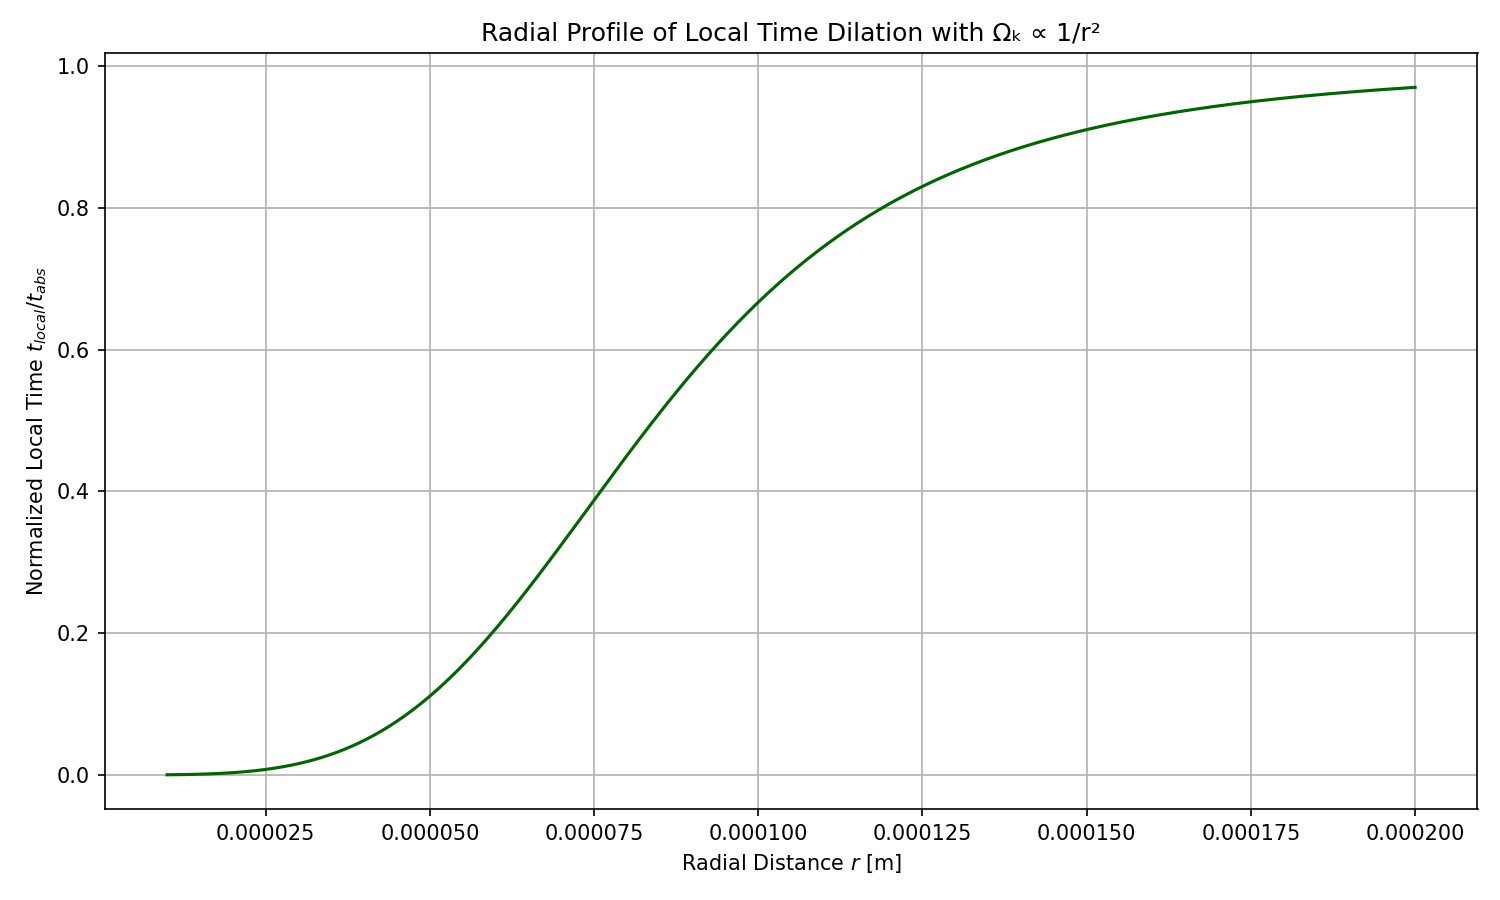
\includegraphics[width=0.7\textwidth]{images/02-RadialProfileOfLocalTimeDilation_Radial_LocalTime_Dilation}
  \caption{Radial time dilation profile due to vortex swirl velocity \( v_\varphi(r) = \kappa / r \). The reduction in local clock rate \(\frac{d\tau}{dt}\) scales with \(1/r^2\), and asymptotically approaches 1 at large distances.}
  \label{fig:radial_time_dilation}
\end{figure}

\begin{table}[H]
    \centering
    \begin{tabular}{|c|c|c|}
        \hline
        \textbf{From} & \textbf{To} & \textbf{Conversion Formula} \\
        \hline
        $\bar{t}$ & $\tau$ & $\frac{d\tau}{d\bar{t}} = \omega_{\text{obs}} / \omega_0$ \\
        $\bar{t}$ & $T_v$ & $T_v = \oint \frac{dl}{v_\varphi(r)}$ \\
        $\tau$ & $S(t)$ & $S(t) = \int \Omega(r(t))\, d\tau$ \\
        $\mathcal{N}$ & $T_v$ & $T_v = \int_0^{\mathcal{N}} \chi(r) \, d\mathcal{N}$ (if using \textit{general time-chirality function}) \\
        \hline
    \end{tabular}
    \caption{Sample conversions between Temporal Ontology layers in VAM}
\end{table}

\subsection{GR vs VAM: Temporal Flow and Causality}

For comparison, in general relativity (GR), gravitational time dilation arises from spacetime curvature, expressed by the Schwarzschild metric~\cite{schutz2009first}:
\begin{equation}\label{eq:GRtime}
\frac{d\tau}{dt} = \sqrt{1 - \frac{2GM}{rc^2}}
\end{equation}

The similarities and differences are immediately apparent: GR's gravitational time dilation is related to mass $M$ and gravitational constant $G$, while VAM time dilation is purely hydrodynamic and directly connected to the local rotational velocity of the æther medium via vortex circulation $\kappa$.

\begin{figure}[ht!]
    \centering
    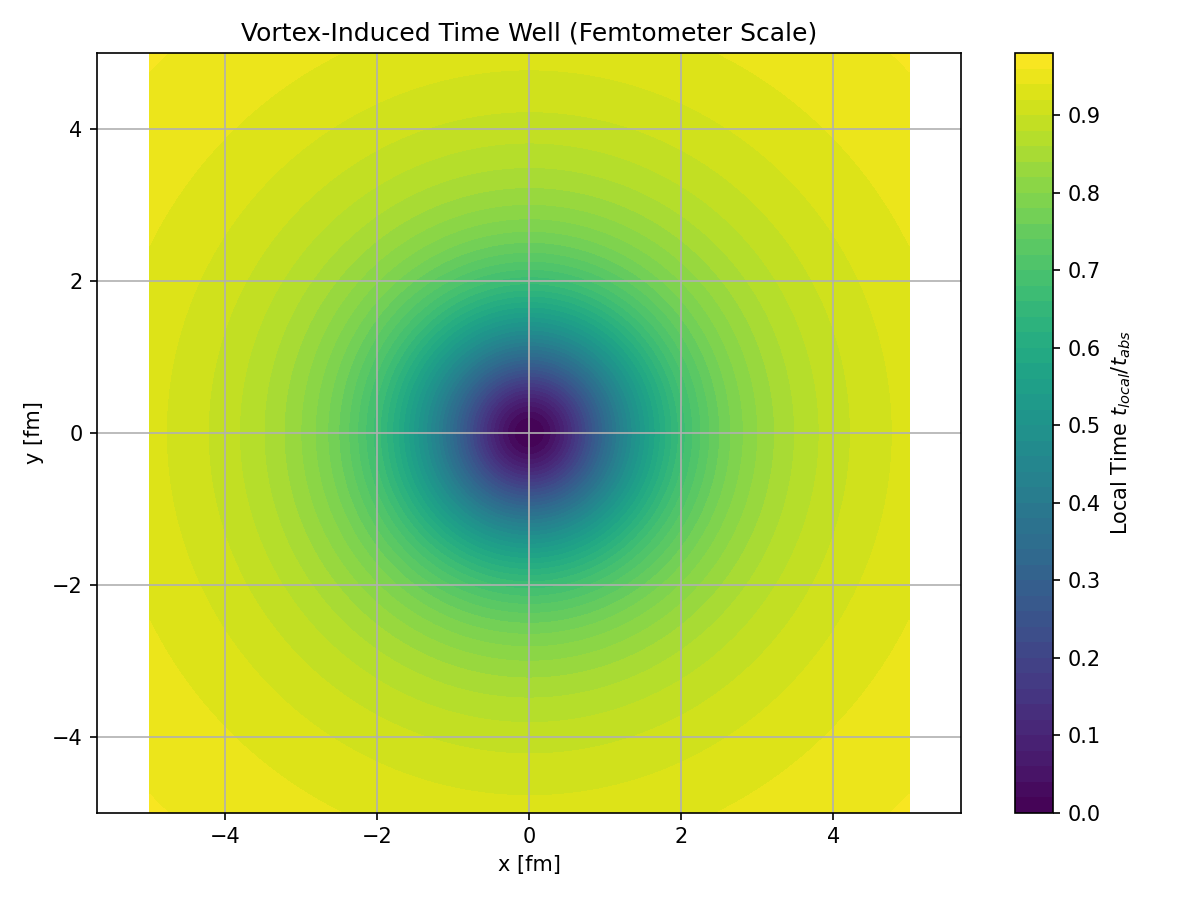
\includegraphics[width=0.7\linewidth]{images/02-RadialProfileOfLocalTimeDilation_Vortex-Induced_Time_Well}
    \caption{Comparison of VAM (vortex dynamics) and GR time dilation, as a function of distance to vortex core and Schwarzschild radius.}
    \label{fig:compare_VAMGR}
\end{figure}

In Figure~\ref{fig:compare_VAMGR} we see that VAM time dilation is functionally comparable to GR prediction at sufficient distance. At decreasing distance (near vortex core or Schwarzschild radius) differences arise due to vortex-specific effects and topological node structures.

In summary, the VAM replaces spacetime curvature with eddy dynamics, while preserving measurable time dilation effects consistent with established experimental results such as Hafele–Keating~\cite{hafele1972around}, but from a fundamentally different physical explanation.

For illustration, in Figure~\ref{fig:comparisonVAMGR} we explicitly compare VAM and GR for a neutron star with $M = 2\,M_\odot$ and radius $R = 10\,\text{km}$. The differences become clear near the surface of the object, where vortex-specific effects occur.

\begin{figure}[ht!]
    \centering
    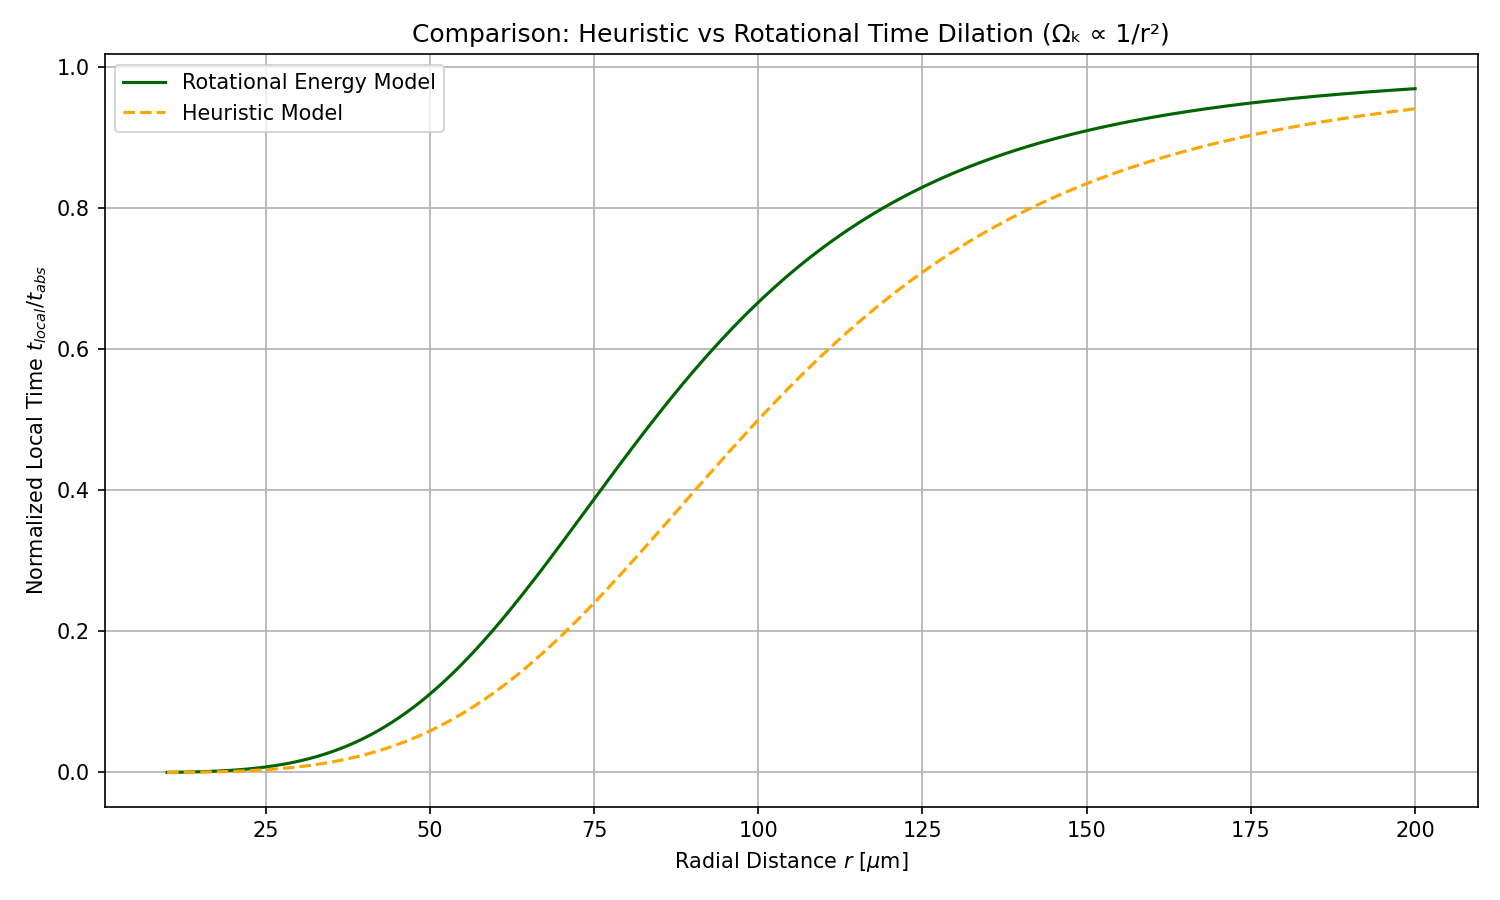
\includegraphics[width=0.7\linewidth]{images/04-RotationalVsHeuristicTimeDilation}
    \caption{Difference between VAM and GR time dilation for a neutron star ($2\,M_\odot$, $R=10$ km).}
    \label{fig:comparisonVAMGR}
\end{figure}

\subsection{Practical implications and experimental testability}

A practical implication of vortex-induced time dilation is that clocks would run measurably slower close to intense vortex fields. This can be tested theoretically with ultra-precise atomic clocks in laboratory vortex experiments, or indirectly via astrophysical observations of pulsars and neutron stars. The Hafele–Keating experiment provides a direct analogy for time dilation due to motion and height differences, which in VAM corresponds to local vortex variations~\cite{hafele1972around}.

\begin{figure}[ht!]
    \centering
    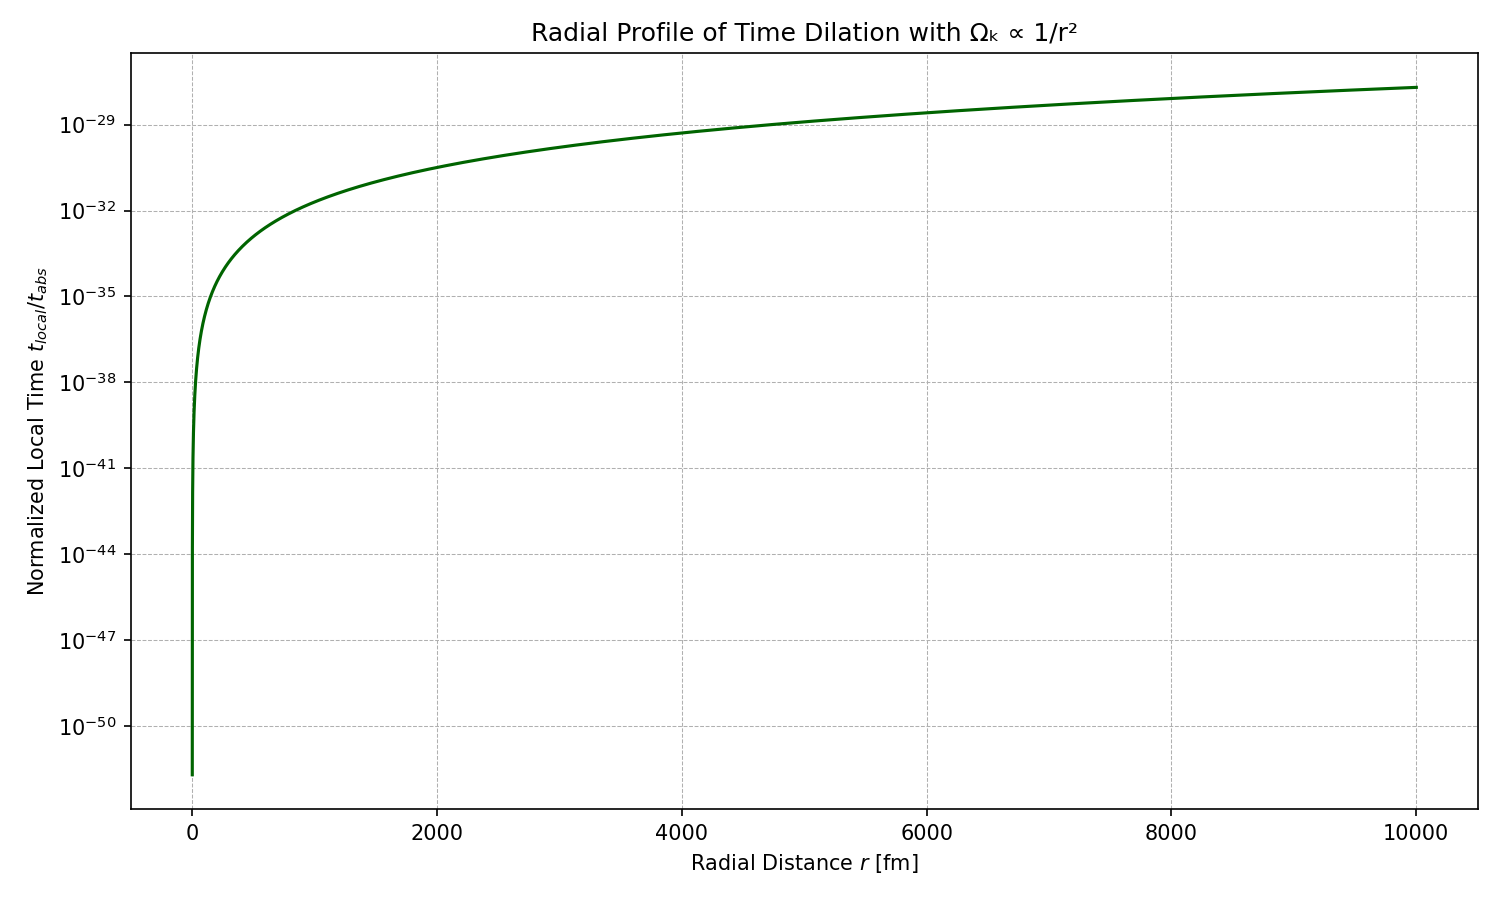
\includegraphics[width=0.7\linewidth]{images/05-LogarithmicDecayLocalTime}
    \caption{Extended radial time dilation profile with $\Omega_k \propto 1/r^2$, showing deep time well characteristics of vortex fields at large radius.}
    \label{fig:NewGraph}
\end{figure}